\documentclass[12pt]{article}
\usepackage{amsmath,amsfonts,amsthm,amssymb}
\usepackage{setspace}
\usepackage{fancyhdr}
\usepackage{lastpage}
\usepackage{extramarks}
\usepackage[ruled,vlined]{algorithm2e}
\usepackage{chngpage}
\usepackage{soul,color}
\usepackage{graphicx,float,wrapfig}
\usepackage{listings}
\lstset{
    basicstyle=\ttfamily,
    mathescape
}
\usepackage{hyperref}

\RequirePackage{amssymb, amsfonts, amsmath, latexsym, verbatim, xspace, setspace}
\RequirePackage{tikz, pgflibraryplotmarks}
%\usepackage{algorithm}
\usepackage{subcaption}
\usepackage{algorithmicx}
\usepackage[noend]{algpseudocode}
% honor
\usepackage{booktabs}
\usepackage{array}% http://ctan.org/pkg/array
\newcolumntype{M}{>{\centering\arraybackslash}m{\dimexpr.25\linewidth-2\tabcolsep}}
%

\usepackage{enumitem}
\usepackage[parfill]{parskip} % put space between paragraphs
\setlist{listparindent=\parindent} % make paragraphs in lists normal
\usepackage{xcolor}

\newcommand{\Class}{ \normalsize CS 331: Algorithms and Complexity (Spring 2024)\\
\small    Unique Number: 50930, 50935 50940, 50945
}


\def\changemargin#1#2{\list{}{\rightmargin#2\leftmargin#1}\item[]}
\let\endchangemargin=\endlist

%\newcommand{\ClassInstructor}{Fares}
%\newcommand{\ClassInstructor}{Fares}

\def\changemargin#1#2{\list{}{\rightmargin#2\leftmargin#1}\item[]}
\let\endchangemargin=\endlist


%\newcommand{\ClassInstructor}{Fares}
% Homework Specific Information. Change it to your own
\newcommand{\Title}{Assignment 5}
\newcommand{\DueDate}{Tuesday, 5 March, by 11.59pm}

\newcommand{\StudentName}{}
\newcommand{\StudentClass}{}
\newcommand{\StudentNumber}{}

% In case you need to adjust margins:
\topmargin=-0.45in      %
\evensidemargin=0in     %
\oddsidemargin=0in      %
\textwidth=6.5in        %
\textheight=9.0in       %
\headsep=0.25in         %

% Setup the header and footer
\pagestyle{fancy}                                                       %
\lhead{\StudentName}                                                 %
\chead{\Title}  %
\rhead{\firstxmark}                                                     %
\lfoot{\lastxmark}                                                      %
\cfoot{}                                                                %
\rfoot{Page\ \thepage\ of\ \protect\pageref{LastPage}}                          %
\renewcommand\headrulewidth{0.4pt}                                      %
\renewcommand\footrulewidth{0.4pt}                                      %

%%%%%%%%%%%%%%%%%%%%%%%%%%%%%%%%%%%%%%%%%%%%%%%%%%%%%%%%%%%%%
% Some tools
\newcommand{\enterProblemHeader}[1]{\nobreak\extramarks{#1}{#1 continued on next page\ldots}\nobreak%
\nobreak\extramarks{#1 (continued)}{#1 continued on next page\ldots}\nobreak}%
\newcommand{\exitProblemHeader}[1]{\nobreak\extramarks{#1 (continued)}{#1 continued on next page
\ldots}\nobreak%
\nobreak\extramarks{#1}{}\nobreak}%

%\definecolor{problemStatementColor}{gray}{0.4}
%\definecolor{problemSolutionColor}{gray}{0}
\newcommand{\homeworkProblemName}{}%
\newcounter{homeworkProblemCounter}%
\newenvironment{homeworkProblem}[1][Problem \arabic{homeworkProblemCounter}]%
{\stepcounter{homeworkProblemCounter}%
\renewcommand{\homeworkProblemName}{#1}%
\section*{\homeworkProblemName}%
\enterProblemHeader{\homeworkProblemName}
%\color{problemStatementColor}
}%
{\exitProblemHeader{\homeworkProblemName}}%

\newcommand{\homeworkSectionName}{}%
\newlength{\homeworkSectionLabelLength}{}%
\newenvironment{homeworkSection}[1]%
{% We put this space here to make sure we're not connected to the above.

    \renewcommand{\homeworkSectionName}{#1}%
    \settowidth{\homeworkSectionLabelLength}{\homeworkSectionName}%
    \addtolength{\homeworkSectionLabelLength}{0.25in}%
    \changetext{}{-\homeworkSectionLabelLength}{}{}{}%
    \subsection*{\homeworkSectionName}%
    \enterProblemHeader{\homeworkProblemName\ [\homeworkSectionName]}}%
    {\enterProblemHeader{\homeworkProblemName}%

    % We put the blank space above in order to make sure this margin
    % change doesn't happen too soon.
    \changetext{}{+\homeworkSectionLabelLength}{}{}{}}%

\newcommand{\partialSolution}{\textbf{Partial solution:} }
\newcommand{\solution}{\textbf{Solution:} }
\newcommand{\Acknowledgement}[1]{\ \\{\bf Acknowledgement:} #1}

\newcommand{\maxpt}[1]{\ifthenelse{\equal{#1}{1}}{\textbf{(#1 pt)}}{\textbf{(#1 pts)}}}
%%%%%%%%%%%%%%%%%%%%%%%%%%%%%%%%%%%%%%%%%%%%%%%%%%%%%%%%%%%%%


\DeclareMathOperator{\opt}{OPT}
\setlist[enumerate,1]{label=\bfseries(\alph*)}
%%%%%%%%%%%%%%%%%%%%%%%%%%%%%%%%%%%%%%%%%%%%%%%%%%%%%%%%%%%%%
% Make title
\title{\textmd{\bf \Class\\ \Title}\\\vspace{0.1in}\small{Due\ on\ \DueDate}}
\date{}
\author{\textbf{\StudentName}\ \ \StudentClass\ \ \StudentNumber}
%%%%%%%%%%%%%%%%%%%%%%%%%%%%%%%%%%%%%%%%%%%%%%%%%%%%%%%%%%%%%

\begin{document}
    \maketitle \thispagestyle{empty}


    %%%%%%%%%%%%%%%%%%%%%%%%%%%%%%%%%%%%%%%%%%%%%%%%%%%%%%%%%%%%%
    % Begin edit from here

    \maketitle \thispagestyle{empty}

    %		\begin{figure}[h]
    %			\centering
    %			\includegraphics[width=0.75\textwidth]{../HonorCode}
    %		\end{figure}
    %
    %		\begin{changemargin}{1 in}{1 in}
    %			We are giving you these solutions as review material to help you study
    %			for the rest of the course. Please do not share them with
    %			future students of CS 331 or post them on external sites.
    %		\end{changemargin}

    %		\newpage

    %%%%%%%%%%%%%%%%%%%%%%%%%%%%%%%%%%%%%%%%%%%%%%%%%%%%%%%%%%%%%
    % Begin edit from here
    \begin{homeworkProblem}[Problem 1]
        \maxpt{8}
        \begin{enumerate}
            \item \maxpt{6}\\
            A naive solution would be to split into 3 cases, one for each of the 3 possible
            operations\\
            (1) Including characters in both strings(Until no more characters in one of the
            strings)\\
            (2) Include character of first string and add gap to second string(Until no more
            characters in first string)\\
            (3) Include character of second string and add gap to first string(Until no more
            characters in second string)\\
            OPT(i, j) = min($\alpha_{x_i y_i} + OPT(i - 1, j - 1)$, $\delta + OPT(i - 1, j)$,
            $\delta + OPT(i, j - 1)$)\\
            This yields a time complexity of $O(3^{m + n})$\\
            Example: String$_1$: CH, String$_2$: EN\\
            We have 3 possibilities for our first layer, (C, E), (C, \_), (\_, E)\\
            \begin{tikzpicture}
            [
                level 1/.style={sibling distance=60mm},
                level 2/.style={sibling distance=35mm},
                level 3/.style={sibling distance=30mm},
                level 4/.style={sibling distance=30mm}
            ]
                \node{(C, E)}
                child {
                    node {(CH, EN)}}
                child {
                    node {(CH, E\_)}
                    child {node {(CH\_, E\_N)}}
                }
                child {
                    node {(C\_, EN)}
                    child {node {(C\_H, EN\_)}}
                };
            \end{tikzpicture}\\
            We have 3 leaves, (CH, EN), (CH\_, E\_N), (C\_H, EN\_)\\
            \begin{tikzpicture}
            [
                level 1/.style={sibling distance=60mm},
                level 2/.style={sibling distance=35mm},
                level 3/.style={sibling distance=30mm},
                level 4/.style={sibling distance=30mm}
            ]
                \node{(C, \_)}
                child {
                    node {(CH, \_E)}
                    child {node {(CH\_, \_EN)}}
                }
                child {
                    node {(CH, \_\_)}
                    child {
                        node {(CH\_, \_\_E)}
                        child {node {(CH\_\_, \_\_EN)}}
                    }
                }
                child {
                    node {(C\_, \_E)}
                    child {node {(C\_H, \_EN)}}
                    child {
                        node {(C\_H, \_E\_)}
                        child {node {(C\_H\_, \_E\_N)}}
                    }
                    child {
                        node {(C\_\_, \_EN)}
                        child {node {(C\_\_H, \_EN\_)}}
                    }
                };
            \end{tikzpicture}\\
            We have 5 leaves, (CH\_, \_EN), (C\_H, \_EN), (C\_H\_, \_E\_N), (C\_\_H, \_EN\_)\\
            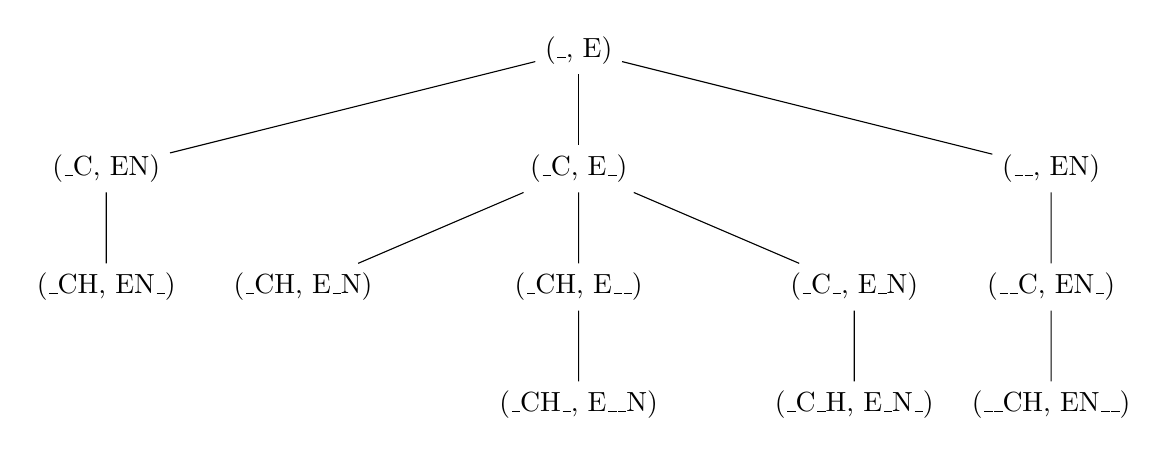
\begin{tikzpicture}
            [
                level 1/.style={sibling distance=60mm},
                level 2/.style={sibling distance=35mm},
                level 3/.style={sibling distance=30mm},
                level 4/.style={sibling distance=30mm}
            ]
                \node{(\_, E)}
                child {
                    node {(\_C, EN)}
                    child {node {(\_CH, EN\_)}}
                }
                child {
                    node {(\_C, E\_)}
                    child {node {(\_CH, E\_N)}}
                    child {
                        node {(\_CH, E\_\_)}
                        child {node {(\_CH\_, E\_\_N)}}
                    }
                    child {
                        node {(\_C\_, E\_N)}
                        child {node {(\_C\_H, E\_N\_)}}
                    }
                }
                child {
                    node {(\_\_, EN)}
                    child {
                        node {(\_\_C, EN\_)}
                        child {node {(\_\_CH, EN\_\_)}}
                    }
                };
            \end{tikzpicture}\\
            We have 5 leaves, (\_CH, EN\_), (\_CH, E\_N), (\_CH\_, E\_\_N), (\_C\_H, E\_N\_), (\_\_CH, EN\_\_)\\
            % TODO
            \item \maxpt{2}
            \begin{itemize}
                \item [1.]
                \begin{tabular}{|c|c|c|c|c|}
                    \hline
                    \_ & A & L & G & O \\
                    \hline
                    T  & 1 & 2 & 3 & 4 \\
                    \hline
                    E  & 2 & 2 & 3 & 4 \\
                    \hline
                    S  & 3 & 3 & 3 & 4 \\
                    \hline
                    T  & 4 & 4 & 4 & 4 \\
                    \hline
                \end{tabular}\\
                The optimal alignment is zero gaps:\\
                $Alignment_1$: ALGO\\
                $Alignment_2$: TEST\\
                % TODO
                \item [2.]
                The cost is the value in the bottom right corner, 4\\
                Cost is 4 since there are 4 sets of characters that are different
                % TODO
            \end{itemize}
        \end{enumerate}
    \end{homeworkProblem}

    \begin{homeworkProblem}[Problem 2]
        \maxpt{12}
        \begin{enumerate}
            \item
            Indices (i, j) store the minimum number of cuts needed to make the substring from i
            to j a set of palindromes.\\
            \begin{lstlisting}
def min_palindrome(s):
    sections = [$\infty$] * len(s)
    for j in [1, len(s)]:
        min_sections = j
        for i in [1, j]:
            if isPali(i, j):
                min_sections = min(min_sections, sections[i - 1] + 1)
        sections[j] = min_sections
            \end{lstlisting}
            I'll test by running it on the string \textquoteleft coffee\textquoteright\\
            Each iteration runs with a fixed endpoint j and a increasing start point i.\\
            First iteration: ($1\to 1$, 1)
            \begin{tabular}{|c|c|c|c|c|c|c|}
                \hline
                $1$ & $\infty$ & $\infty$ & $\infty$ & $\infty$ & $\infty$ \\
                \hline
            \end{tabular}\\
            Second iteration: ($1\to 2$, 2)
            \begin{tabular}{|c|c|c|c|c|c|c|}
                \hline
                $1$ & $2$ & $\infty$ & $\infty$ & $\infty$ & $\infty$ \\
                \hline
            \end{tabular}\\
            Third iteration: ($1\to 3$, 3)
            \begin{tabular}{|c|c|c|c|c|c|c|}
                \hline
                $1$ & $2$ & $3$ & $\infty$ & $\infty$ & $\infty$ \\
                \hline
            \end{tabular}\\
            Fourth iteration: ($1\to 4$, 4)
            \begin{tabular}{|c|c|c|c|c|c|c|}
                \hline
                $1$ & $2$ & $3$ & $3$ & $\infty$ & $\infty$ \\
                \hline
            \end{tabular}\\
            Fifth iteration: ($1\to 5$, 5)
            \begin{tabular}{|c|c|c|c|c|c|c|}
                \hline
                $1$ & $2$ & $3$ & $3$ & $4$ & $\infty$ \\
                \hline
            \end{tabular}\\
            Sixth iteration: ($1\to 6$, 6)
            \begin{tabular}{|c|c|c|c|c|c|c|}
                \hline
                $1$ & $2$ & $3$ & $3$ & $4$ & $4$ \\
                \hline
            \end{tabular}\\
            Let $n = w.length$\\
            The time complexity is $O(n^2)$, as each iteration of the outer
            loop goes from i + 1 to the end of the array, resulting in $\sum\limits_{j=1}^{n} j$\\
            % TODO
            \item
            Assume S is 1-indexed\\
            We either add the new character as a standalone or use it as a palindrome with the
            previous characters in the string.\\
            OPT(i) = min(OPT(i - 1) + 1, min(OPT(j - 1) + 1 for j in [1, i - 1] if isPali(j, i)))\\
            Claim: sections[i] = minimum palindromic substrings of [1, i]\\
            Base Case: i = 1\\
            Our algorithm is correct since for the single first character, it'll return 1\\
            By definition, OPT(1) = 1 = f(1)\\
            Therefore, our base case is correct\\
            Inductive Step: Assume f(i) = OPT(i) = sections[i] for all i $\leq$ k\\
            Show f(k + 1) is correct\\
            We know OPT(k + 1) = min(OPT(k) + 1, min(OPT(j - 1) + 1 for j in [1, k] if isPali(j,
            k + 1)))\\
            f(k + 1) = min(sections[i - 1] + 1) for i in [1, k + 1] if isPali(i, k + 1)\\
            These are the same, so our algorithm is correct\\
            Therefore, our algorithm produces the optimal solution\\
            % TODO
        \end{enumerate}
    \end{homeworkProblem}

    \begin{homeworkProblem}
        \maxpt{10}
        \begin{enumerate}
            \item
            Since we can't include the direct children of a manager, then we need to include
            subtrees another layer deeper.\\
            The optimal solution could be to include the current person, but if the manager was
            accounted for, more enjoyment could be gained.\\
            This isn't greedy since local best choices don't always lead to the global best
            choice.\\
            % TODO
            \item
            I used memoization to store the maximum enjoyment for each person.\\
            The idea is to store the two maximum enjoyments for each person in a map, one for the
            person potentially included in the enjoyment and one for the person not allowed in the
            enjoyment.\\
            $e_i$ = enjoyment if person can be included and its associated list of people\\
            $e_e$ = enjoyment if person can't be included and its associated list of people\\
            \begin{lstlisting}
Map(person, {true: $e_i$, false: $e_e$}) = {}
def max_enjoyment(person, canInclude) -> int:
    if person in Map:
        return Map(person, canInclude)

    ci = person.enjoyment
    for child in person.children:
        ci += max_enjoyment(child, false)

    ce = 0
    for child in person.children:
        ce += max_enjoyment(child, true)
    Map(person, {ci, ce})
    return canInclude ? max(ci, ce) : ce
            \end{lstlisting}
            Let i be the level where i = 0 is the bottom most person\\
            The optimal solution is OPT(i) = max(sum(OPT(i - 1)), sum(OPT(i - 2)) + enjoyment$_i$)\\
            We compute each peron's enjoyment included and excluded once, so the time complexity
            is $O(n)$, where n = number of people\\
            Now, I'll show the algorithm is optimal\\
            Base Case: person is bottom of tree, show f(0) = OPT(0)\\
            Then, $e_i$ = person.enjoyment and $e_e$ = 0\\
            This is optimal since OPT(i) = max(sum(0), sum(0) + enjoyment$_i$) = max(0, enjoyment$_i$) = enjoyment$_i$\\
            Therefore, our base case is correct\\
            Inductive Hypothesis: Assume f(i) = OPT(i) for i $\leq$ k\\
            Inductive Step: Show f(k + 1) = OPT(k + 1)\\
            Our algorithm computes sum(f(k)) and sum(f(k - 1)) + enjoyment$_{k + 1}$\\
            It then returns the maximum of the two since we allow the inclusion of the current
            person\\
            OPT(k + 1) = max(sum(OPT(k)), sum(OPT(k - 1)) + enjoyment$_{k + 1}$)\\
            Therefore, the two are the same, so our algorithm is correct\\
            Therefore, our algorithm produces the optimal solution\\
            % TODO
        \end{enumerate}
    \end{homeworkProblem}

\end{document}
